\documentclass[oneside,onecolumn]{article}


\usepackage{blindtext} % Package to generate dummy text throughout this template 

\usepackage[sc]{mathpazo} % Use the Palatino font
\usepackage[T1]{fontenc} % Use 8-bit encoding that has 256 glyphs
\linespread{1.05} % Line spacing - Palatino needs more space between lines
\usepackage{microtype} % Slightly tweak font spacing for aesthetics

\usepackage[english]{babel} % Language hyphenation and typographical rules

\usepackage[hmarginratio=1:1,top=32mm,columnsep=20pt]{geometry} % Document margins
\usepackage[hang, small,labelfont=bf,up,textfont=it,up]{caption} % Custom captions under/above floats in tables or figures
\usepackage{booktabs} % Horizontal rules in tables

\usepackage{lettrine} % The lettrine is the first enlarged letter at the beginning of the text

\usepackage{enumitem} % Customized lists
\setlist[itemize]{noitemsep} % Make itemize lists more compact

\usepackage{abstract} % Allows abstract customization
\renewcommand{\abstractnamefont}{\normalfont\bfseries} % Set the "Abstract" text to bold
\renewcommand{\abstracttextfont}{\normalfont\small\itshape} % Set the abstract itself to small italic text

\usepackage{titlesec} % Allows customization of titles
\renewcommand\thesection{\Roman{section}} % Roman numerals for the sections
\renewcommand\thesubsection{\roman{subsection}} % roman numerals for subsections
\titleformat{\section}[block]{\large\scshape\centering}{\thesection.}{1em}{} % Change the look of the section titles
\titleformat{\subsection}[block]{\large}{\thesubsection.}{1em}{} % Change the look of the section titles

\usepackage{fancyhdr} % Headers and footers
\pagestyle{fancy} % All pages have headers and footers
\fancyhead{} % Blank out the default header
\fancyfoot{} % Blank out the default footer
% \fancyhead[C]{Running title $\bullet$ May 2016 $\bullet$ Vol. XXI, No. 1} % Custom header text
\fancyfoot[RO,L]{\thepage} % Custom footer text

\usepackage{titling} % Customizing the title section

\usepackage{hyperref} % For hyperlinks in the PDF

\usepackage{romannum} % Roman numbers 
\usepackage{graphicx}
\usepackage{wrapfig}
\graphicspath{ {images/} }
\usepackage{wrapfig}
\usepackage{subcaption}

% ----------------------------------------------------------------------------------------
%	TITLE SECTION
% ----------------------------------------------------------------------------------------

\setlength{\droptitle}{-4\baselineskip} % Move the title up

\pretitle{\begin{center}\Huge\bfseries} % Article title formatting
  \posttitle{\end{center}} % Article title closing formatting
\title{Motion planning of a fixed wings Uav through an hybrid approach based on artificial potential
  fields and RRT. } % Article title
\author{%
  \textsc{Edoardo Ghini} \\[1ex] % Your name
  \normalsize \href{mailto:ghiniedoardo@gmail.com}{ghiniedoardo@gmail.com} % Your email address
  \and % Uncomment if 2 authors are required, duplicate these 4 lines if more
  \textsc{Gianluca Cerilli} \\[1ex] % Second author's name
  \normalsize \href{mailto:gianlucer@gmail.com}{gianlucer@gmail.com}\\ % Second author's email address
  \normalsize Dipartimento di Ingegneria dell'Universita di Roma La Sapienza\\
}
\date{\today} % Leave empty to omit a date
% \renewcommand{\maketitlehookd}{%
% \begin{abstract}
%   \noindent  This is the abstract, try to be concise !
% \end{abstract}
% }
%   ----------------------------------------------------------------------------------------

\begin{document}

% Print the title
\maketitle
\bigskip
\bigskip
\bigskip
\bigskip
\begin{center}
  
\includegraphics[width=0.3\textwidth]{laSapienza}
\end{center}


% ----------------------------------------------------------------------------------------
%	ARTICLE CONTENTS
% ----------------------------------------------------------------------------------------
\newpage
\section{Introduction}

\lettrine[nindent=0em,lines=3]{W}e will present a work made
for an international challenge\footnote{The challenge is the AUVSI-SUAS hosted
  in united states in summer 2018.} that every year involves several accademic teams.\\
This report respects the following structure : \\
in section \Romannum{2}, we will present the problem statement and in section
\Romannum{3} we will give tecnical informations on the hardware at our disposal,
finally in section \Romannum{4}, the adopted solution will be discussed.

% ------------------------------------------------

\section{Problem Statement}
All the joining teams to the challenge will have to compete on several tasks
concerning on actual problems in the governance of Unmanned Aerial Vehicles.\\
Each team will bring its prototype of UAV on a common flight ground and try to
score the greatest number of points among all the tasks proposed which are:
\begin{enumerate}\centering
\item Autonomous Flight
\item Obstacle Avoidance
\item Object Detection
\item Object Classification
\item Object Localization 
\item Air Delivery
\end{enumerate}


This will be the first partecipation at a competition of this kind for the team
Sapienza, in fact the previous challenges in which our university has already
been involved required a human controlled guidance system.
Therefore the autonomous flight constraint has to be faced without previous
insights on the matter.
\newpage

\subsection{Starting Points}
The areonautical research department, in the past decade, has spent a big
effort working to an autonomous guidance system, that has been thinkered,
designed and implemented by master students in theyr thesis.\\
This system allows to control the complex aerodynamics of the vehicle from an
higher level of abstraction, its main high level control mode uses a series of
way points that describes a trajectory.\\
\bigskip
\begin{wrapfigure}{r}{5.5cm}
  \caption{YAK scaled aero model}\label{wrap-fig:1}
  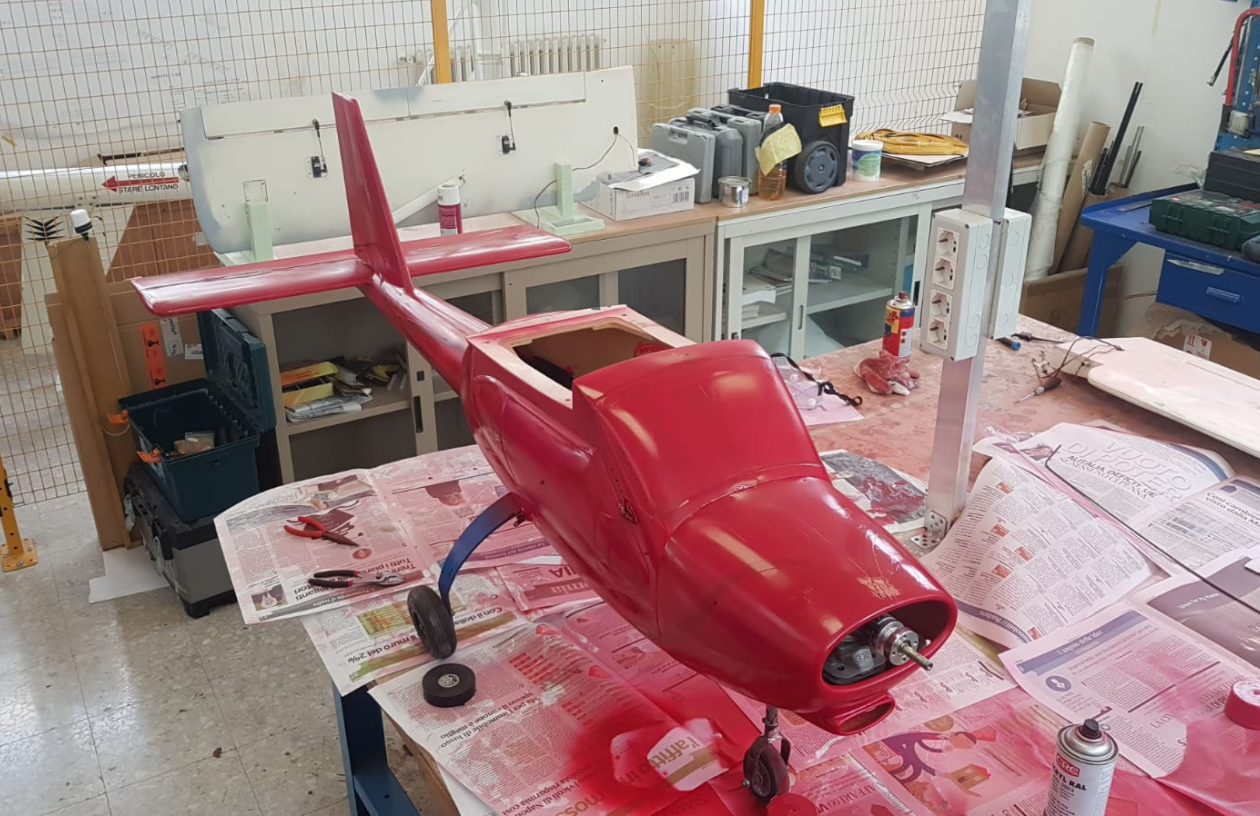
\includegraphics[width=5.5cm]{YAK1}
\end{wrapfigure} 

In this way the aircraft will likely follow a path made of lines that intersects subsequent waypoints.\\
The system is designed to work on an on-board computer and to communicate with a
ground station that will continuously send to and receive from the judges's
server, telemetrical data and mission objectives.\\
We will use a fixed-wigs radio controlled aircraft model\footnote{It is a scaled
  reproduction (1:3 ratio) of the YAK 112} commonly used in hobby
modeling as shown in Figure~\ref{wrap-fig:1}.


\subsection{Our task}
As atomic part of the team which counts several members coming from an
aeronutical background, we have an uncommon area of expertise that concerns
\textbf{automation} and \textbf{robotics}.\\ So we engaged the autonomous guidance problem that
comprehend also the obstacle avoidance clause.\par
The competition will be organized in such a way that during the various missions
of the challenge each team will receive pose informations about fixed and mobile
obstacles that will be \textbf{virtual}.\\
Then the judges will check the success or failure in avoiding obstacles
according to the \textbf{telemetry} data that they will receive from each team.\\
In other words, we where supposed to design a \textbf{path planning} algorith
that will bring the UAV from a start position to a goal position without collisions.




\section{Hardware components}

\subsection{Propulsion}
\begin{wrapfigure}{r}{5.5cm}
  \caption{DLE55 motor}\label{wrap-fig:2}
  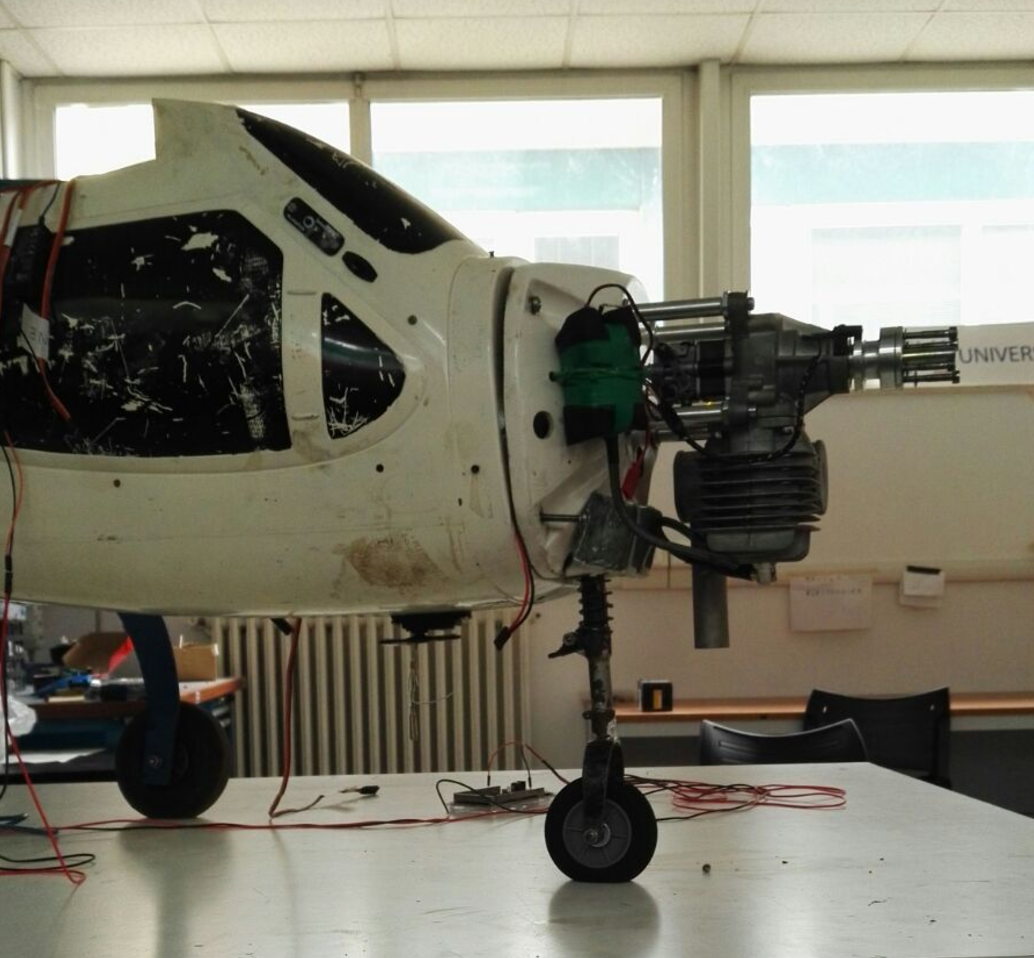
\includegraphics[width=5.5cm]{YAK3}
\end{wrapfigure} 



The engine chosen is a \textbf{DLE55} (in Figure~\ref{wrap-fig:2} ) :

\begin{enumerate}
\item 50 cc monocylinder petrol engine
\item reservoir capable of containing 950cc of petrol
\item Equipped with a 7, 4V LiPo battery
\end{enumerate}


\subsection{On board computing}
The autonomous guidance architecture, implemented in Matlab and Simulink, is
converted in compiled high speed C, Cpp language.\\ It will be run by Arduino Due
and there will be also a Raspberry pi Model 3 that will run a kalman filter in
order to process all signals from sensors.

\bigskip I am arrived here  % TODO at the end we will focus on layouts and image positions


\subsection{Sensing instruments}
Maecenas sed ultricies felis. Sed imperdiet dictum arcu a egestas. 
\subsection{Communication devices}
Maecenas sed ultricies felis. Sed imperdiet dictum arcu a egestas. 
\subsection{Auto pilot framework}
Maecenas sed ultricies felis. Sed imperdiet dictum arcu a egestas. 
\section{Hybrid planner}
We implemented two different strategies, since both present some shortcomings
and advantages, we tried to take the best of the two worlds

\subsection{RRT}
RRT (Rapidly-exploring Random Tree) is a probabilistic planner that randomly builds a space-building tree.\\
It has been used offline considering some motion primitives (produced by some specific velocity inputs) to define a path for the UAV, biasing it towards the unexplored areas closest to the goal.
\subsection{Artificial potentials}
Artificial Potential Fields (APF) have been considered for two main reasons:
\begin{itemize}
\item the world can be approximated to a "world of spheres" (since there are cylindrical obstacles that we consider in 2D), that prevents the UAV entering the basin of attraction of some local minima
\item when the UAV faces an obstacle, RRT must expand many branches before getting around it. This leads to a significant slowdown
\end{itemize}
Using APF the UAV can react as soon as entering the range of influence of the obstacle, with a smooth movement. This also because an implementation with vertex fields has been made, replacing repulsive actions with actions forcing the robot to get around it.
\subsection{Implementation}
We consider the kinematic model of a fixed-wing UAV flying at a constant altitude. So, we can neglect the pitch angle, obtaining:\\
\begin{array}{lcc}
  $ \dot{x} $ & = & $vcos \psi $ \\
  $ \dot{y} $ & = & $vsin \psi $ \\
  $ \dot{\psi} $ & = & -$ \frac{g}{v} tan \phi $ \\
  $ \dot{\phi} $ & = & $ u_{\phi } $
\end{array}\\
in which the speed $v$ and roll rate $u_{\phi}$ are the control inputs.

%% \footnote{Example footnote}.

% ------------------------------------------------

\section{Conclusion}

% \begin{table}
%   \caption{Example table}
%   \centering
%   \begin{tabular}{llr}
      %       \toprule
      %       \multicolumn{2}{c}{Name} \\
      %       \cmidrule(r){1-2}
      %       First name & Last Name & Grade \\
      %       \midrule
      %       John & Doe & $7.5$ \\
      %       Richard & Miles & $2$ \\
      %       \bottomrule
      %     \end{tabular}
      %       \end{table}


\begin{equation}
  \label{eq:emc}
  e = mc^2
\end{equation}


      %       ----------------------------------------------------------------------------------------
      %       REFERENCE LIST
      %       ----------------------------------------------------------------------------------------

\begin{thebibliography}{99} % Bibliography - this is intentionally simple in this template

\bibitem[Figueredo and Wolf, 2009]{Figueredo:2009dg}
  Figueredo, A.~J. and Wolf, P. S.~A. (2009).
  \newblock Assortative pairing and life history strategy - a cross-cultural
  study.
  \newblock {\em Human Nature}, 20:317--330.
  
\end{thebibliography}

      %       ----------------------------------------------------------------------------------------

\end{document}
